\subsubsection{UC 40 - Igienizzazione Postazioni}

\begin{figure}[h]
  \centering
    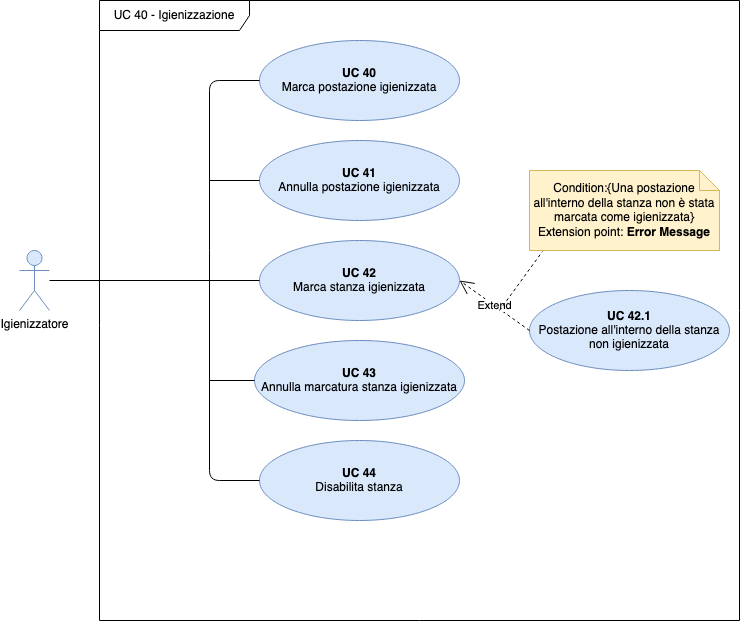
\includegraphics[scale=0.5]{src/CasiDUso/Immagini/UC40.png}
  \caption{UC40  - Igienizzazione postazioni}
\end{figure}

Il presente diagramma vuole riassumere la possibilità di igienizzazione delle postazioni da parte di un utente igienizzatore all'interno dell’applicazione.

\begin{itemize}
\item \textbf{Attori primari:} igienizzatore;
\item \textbf{Descrizione:} l’utente può gestire le stanze e postazioni registrate nell’applicazione a cui ha accesso a livello di permessi, marcando come igienizzate o disabilitando le relative postazioni o intere stanze;
\item \textbf{Precondizione:} ogni utente è autenticato, e naviga nell’apposita sezione di gestione delle postazioni o stanze;
\item \textbf{Postcondizione:} l’utente ha gestito le proprie postazioni o stanze;
\item \textbf{Scenario principale:} 
	\begin{itemize}
		\item l’utente naviga nell’apposita sezione di gestione delle postazioni o stanze;
		\item l’utente marca come igienizzate le postazioni o stanze a cui ha accesso;
	\end{itemize}
\end{itemize}

\subsubsection{UC40.1 - Marca postazione igienizzata}

\begin{itemize}
\item \textbf{Attori primari:} igienizzatore;
\item \textbf{Descrizione:} l'utente può marcare la postazione come igienizzata, servibile quindi dagli utenti;
\item \textbf{Precondizione:} l'utente naviga nell’apposita sezione di gestione della postazione; 
\item \textbf{Postcondizione:} l’utente ha marcato con successo una postazione come igienizzata;
\item \textbf{Scenario principale:} 
	\begin{itemize}
		\item l'utente naviga nell’apposita sezione di gestione della postazione;		
		\item l’utente contrassegna la postazione come igienizzata;
		\item il sistema elabora correttamente la richiesta.
	\end{itemize}
\end{itemize}

\subsubsection{UC40.2 - Annulla postazione igienizzata}

\begin{itemize}
\item \textbf{Attori primari:} igienizzatore;
\item \textbf{Descrizione:} l’igienizzatore può annullare lo stato di postazione igienizzata precedentemente segnato, impostando la postazione come “non igienizzata”;
\item \textbf{Precondizione:} l'utente naviga nell’apposita sezione di gestione della postazione; 
\item \textbf{Postcondizione:} l'utente ha marcato con successo una postazione come non igienizzata;
\item \textbf{Scenario principale:} 
	\begin{itemize}
		\item l’utente naviga nell’apposita sezione di gestione della postazione;		
		\item l’utente annulla lo stato di postazione igienizzata precedentemente assegnato;
		\item il sistema elabora correttamente la richiesta.
		\end{itemize}
\end{itemize}

\subsubsection{UC40.3 - Marca stanza igienizzata}

\begin{itemize}
\item \textbf{Attori primari:} igienizzatore;
\item \textbf{Descrizione:} l’igienizzatore può marcare un'intera stanza come igienizzata, cui ogni postazione al suo interno è sanificata e servibile quindi dagli utenti;
\item \textbf{Precondizione:} l'utente naviga nell’apposita sezione di gestione della stanza; 
\item \textbf{Postcondizione:} l'utente ha marcato con successo una stanza come igienizzata;
\item \textbf{Scenario principale:} 
	\begin{itemize}
		\item l’utente naviga nell’apposita sezione di gestione della stanza;	
		\item l'utente contrassegna la stanza come igienizzata;
		\item il sistema elabora correttamente la richiesta o restituisce un errore, che può essere dovuto ai seguenti fattori:
			\begin {itemize}
				\item una postazione all’interno della stanza non è marcata come igienizzata.
			\end{itemize}
		\end{itemize}
\end{itemize}

\subsubsection{UC40.4 - Marca stanza non igienizzata}

\begin{itemize}
\item \textbf{Attori primari:} igienizzatore;
\item \textbf{Descrizione:} l’igienizzatore può annullare lo stato di stanza igienizzata precedentemente segnato, impostando la stanza come “non igienizzata”;
\item \textbf{Precondizione:} l'utente naviga nell’apposita sezione di gestione della stanza; 
\item \textbf{Postcondizione:} l'utente ha marcato con successo una stanza come non igienizzata;
\item \textbf{Scenario principale:} 
	\begin{itemize}
		\item l’utente naviga nell’apposita sezione di gestione della stanza;	
		\item l'utente contrassegna la stanza come non igienizzata;
		\item il sistema elabora correttamente la richiesta;
	\end{itemize}
\end{itemize}

\subsubsection{UC40.5 - Disabilita stanza}

\begin{itemize}
\item \textbf{Attori primari:} igienizzatore;
\item \textbf{Descrizione:} l’igienizzatore può disabilitare una stanza, impedendo quindi l’accesso a tutti gli utenti registrati alle relative postazioni;
\item \textbf{Precondizione:} l'utente naviga nell’apposita sezione di gestione della stanza; 
\item \textbf{Postcondizione:} l'utente ha marcato con successo una stanza come disabilitata;
\item \textbf{Scenario principale:} 
	\begin{itemize}
		\item l’utente naviga nell’apposita sezione di gestione della stanza;	
		\item l'utente contrassegna la stanza come disabilitata;
		\item il sistema elabora correttamente la richiesta;
	\end{itemize}
\end{itemize}



